
到目前为止,我们已经学习了几个IR单元,如模块、功能、基本模块和指令。我们还学习了一些逻辑单元,如CFG和调用图。本节中,我们将看看一个更符合逻辑的IR单元:循环。

循环是程序员经常使用的结构,更不用说几乎每一种编程语言也包含这个概念。循环重复执行一定数量的指令多次,这为程序员节省了大量自己重复代码的工作。但是,如果循环包含任何效率低下的代码——耗时的内存负载总是传递相同的值——性能下降也会随着迭代的次数而放大。

因此,编译器的工作就是从循环中消除尽可能多的缺陷。除了从循环中移除次优代码,因为循环在运行时性能的关键路径上,人们一直试图通过特殊的基于硬件的加速来进一步优化它们,例如:用向量指令替换循环,可以在几个周期内处理多个标量值。简而言之,循环优化是生成更快、更高效程序的关键。这在高性能和科学计算社区中尤为重要。

本节中,我们将学习如何使用LLVM处理循环。我们将尝试通过两个部分来解决这个问题:

\begin{itemize}
\item LLVM中的循环表示
\item LLVM中的循环设施
\end{itemize}

在LLVM中,循环比其他(逻辑)IR单元稍微复杂一些。因此,我们将首先了解LLVM中循环的高级概念及其术语。然后,第二部分中,我们将接触LLVM中用于处理循环的设施和工具。

让我们从第一部分开始。

\subsubsubsection{10.4.1\hspace{0.2cm}LLVM中的循环表示}

在LLVM中,循环由\texttt{Loop}类表示。这个类可以捕获任何控制流结构,该结构具有来自前块中的封闭基本块的后边[译者:这里的描述有点绕,可以看一下图10.8。]。在深入其细节之前,让我们先学习如何检索\texttt{Loop}实例。

在LLVM IR中,循环是一个逻辑IR单元。也就是说,是从物理IR单位推导(或计算)出来的。这样,我们需要从\texttt{AnalysisManager}中检索计算出的循环实例。下面是如何在\texttt{Pass}函数中检索\texttt{Loop}的例子:

\begin{lstlisting}[style=styleCXX]
#include "llvm/Analysis/LoopInfo.h"
…
PreservedAnalyses run(Function &F, FunctionAnalysisManager
&FAM) {
	LoopInfo &LI = FAM.getResult<LoopAnalysis>(F);
	// `LI` contains ALL `Loop` instances in `F`
	for (Loop *LP : LI) {
		// Working with one of the loops, `LP`
	}
…
}
\end{lstlisting}

\texttt{LoopAnalysis}是一个LLVM分析类,为我们提供了一个\texttt{LoopInfo}实例,包含了一个\texttt{Function}中的所有\texttt{Loop}实例。我们可以遍历一个\texttt{LoopInfo}实例,以获得一个单独的\texttt{Loop}实例。

现在,让我们了解一下\texttt{Loop}实例。

\hspace*{\fill} \\ %插入空行
\noindent
\textbf{循环术语}

一个循环实例包含一个特定循环的多个\texttt{BasicBlock}实例。LLVM为其中一些块以及它们之间的(控制流)边分配了一个特殊的含义/名称。下图显示了这个术语:

\hspace*{\fill} \\ %插入空行
\begin{center}
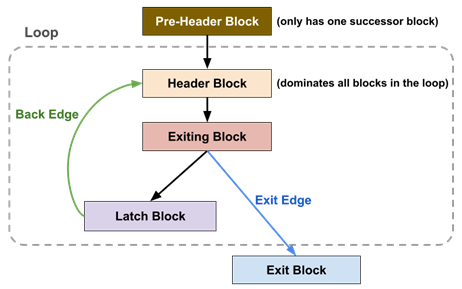
\includegraphics[width=0.8\textwidth]{content/3/chapter10/images/8.png}\\
图10.8 - 循环中的结构和术语
\end{center}

这里,每个矩形都是一个\texttt{BasicBlock}实例。但是,只有在虚线区域内的块才包含在\texttt{Loop}实例中。上图还显示了两个重要的控制流边。让我们详细解释这些术语:

\begin{itemize}
\item \textbf{Header Block}: 这个块标记了一个循环的入口。正式地说,它支配着循环中的所有块,也是Back Edge的目的地。

\item \textbf{Pre-Header Block}: 虽然不是循环的一部分,但表示的是头块作为唯一的后续块。换句话说,它是Header Block的唯一前身。

Pre-header块的存在使得编写一些循环转换变得更容易,例如:当我们想要将一条指令提升到循环的外部,以便它在进入循环之前只执行一次时,Pre-header块可是放置这个指令的好地方。如果没有Pre-header块,则需要为Pre-header块的每一个前身复制这条指令。

\item \textbf{Back Edge}: 这是从循环中的一个块到报头块的控制流边。一个循环可能包含几个Back Edge。

\item \textbf{Latch Block}: 位于后边的源块。

\item \textbf{Exiting Block和Exit Block}: 这两个名称有点令人困惑:Exiting Block是具有控制流边(Exit Edge)的块,从而跳出循环。出口边的另一端,不属于循环的一部分,是Exit Block。一个循环可以包含多个退出块(和出口块)。
\end{itemize}

这些是循环实例中的块的重要术语。除了控制流结构之外,编译器工程师还对可能存在于循环中的一个特殊值感兴趣:\textbf{引导变量}。例如,在下面的代码片段中,变量\texttt{i}是引导变量:

\begin{lstlisting}[style=styleCXX]
for (int i = 0; i < 87; ++i){…}
\end{lstlisting}

循环可能不包含引导变量——C/C++中的许多while循环都没有引导变量。此外,要找出一个引导变量,以及它的边界(开始、结束和停止值)并不总是很容易。下一节中,我们将展示一些工具来帮助我们完成这项任务。但在那之前,我们将讨论一个有趣的话题,关于循环的标准形式。

\hspace*{\fill} \\ %插入空行
\noindent
\textbf{规范循环}

前一节中,我们了解了LLVM中循环的几个术语,包括Pre-header前块。Pre-header块的存在使开发循环转换变得更容易,因为它创建了更简单的循环结构。在这个讨论之后,还有其他一些属性可以让我们更容易地编写循环转换。如果循环实例有这些漂亮的属性,我们通常称它为\textbf{规范循环}。LLVM中的优化流水在将一个循环发送到任何循环转换之前,会尝试将其“更改”成这种规范形式。

目前,LLVM有两种\texttt{Loop}形式:\textbf{简化}和\textbf{旋转}。简化后具有以下属性:

\begin{itemize}
\item 一个Pre-header块。
\item 单一的Back Edge(因此只有单个Latch Block)。
\item 退出块的前身来自循环。换句话说,Header区块支配着所有的出口块。
\end{itemize}

要获得一个简化的循环,可以在原始循环上运行\texttt{LoopSimplfyPass}。此外,可以使用\texttt{Loop::is\\LoopSimplifyForm}方法来检查是否存在\texttt{Loop}。

拥有单一Back Edge的好处包括,可以更容易地分析递归数据流——引导变量。对于最后一个属性,如果每个出口块都由循环控制,那么可以更容易地在不受其他控制流路径干扰的情况下将指令“嵌入”到循环指令中。

让我们看看旋转后的形式。最初,在LLVM的循环优化管道中,旋转形式并不是正式的规范形式。但是随着越来越多的循环传递依赖于它,其就成为“事实上的”规范形式。下面的图表显示了旋转循环的样子:

\hspace*{\fill} \\ %插入空行
\begin{center}
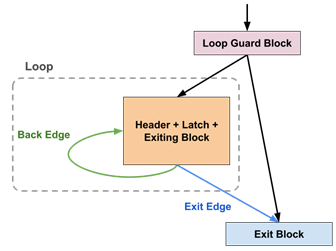
\includegraphics[width=0.9\textwidth]{content/3/chapter10/images/9.png}\\
图10.9  -旋转环路的结构和术语
\end{center}

要获得一个旋转的循环,可以在原始循环上运行\texttt{LoopRotationPass}。要检查一个循环是否旋转,可以使用\texttt{loop::isRotatedForm}方法。

这种旋转后的形式基本上是,将任意循环转换为带有一些额外检查的\texttt{do{…}while(…)}循环(在C/C++中)。假设我们有以下\texttt{for}循环:

\begin{lstlisting}[style=styleCXX]
// `N` is not a constant
for (int i = 0; i < N; ++i){…}
\end{lstlisting}

循环旋转有效地将其转换为以下代码:

\begin{lstlisting}[style=styleCXX]
if (i < N) {
	do {
		…
		++i;
	} while(i < N);
}
\end{lstlisting}

前面代码中显示的边界检查用于确保\texttt{i}变量在一开始就超出边界时,则不执行循环。我们也称其为检查\textbf{循环保护},如上图所示。

除了循环保护,我们还发现旋转循环有一个合并的头、锁存器和退出块。这样做的基本原理是为了确保这个块中的每个指令都有相同的执行计数。这对于编译器优化(如循环向量化)是一个有用的属性。

在此基础上,我们了解了LLVM中的各种循环术语和规范循环的定义。在下一节中,我们将学习一些API,可以帮助我们以一种有效的方式检查这些属性和处理循环。

\subsubsubsection{10.4.2\hspace{0.2cm}LLVM中的循环设施}

在LLVM中了解循环表示的章节节中,我们学习了LLVM IR中循环的高层结构和重要属性。本节中,我们将看到有哪些API可用来检查这些属性,并进一步转换循环。让我们从循环传递开始讨论——应用于\texttt{Loop}实例的LLVM Pass。

在第9章我们了解到有不同种类的LLVM Pass在不同的IR单元上工作——函数和模块的Pass。这两种Pass的运行方法有一个类似的函数签名——LLVM Pass的主要入口点——如下所示:

\begin{lstlisting}[style=styleCXX]
PreservedAnalyses run(<IR unit class> &Unit,
					  <IR unit>AnalysisManager &AM);
\end{lstlisting}

所有\texttt{run}方法都有两个参数—对IR单元实例和\texttt{AnalysisManager}实例的引用。

相反,循环Pass有一个稍微复杂一点的\texttt{run}方法签名,如下所示:

\begin{lstlisting}[style=styleCXX]
PreservedAnalyses run(Loop &LP, LoopAnalysisManager &LAM,
					  LoopStandardAnalysisResults &LAR,
					  LPMUpdater &U);
\end{lstlisting}

\texttt{run}方法有四个参数,但前两个我们已经知道了。以下是对另外两个的描述:

\begin{itemize}
\item 第三个参数,\texttt{LoopStandardAnalysisResults}提供了一些分析数据实例,例如:\texttt{AAResults}(别名分析数据)、\texttt{DominatorTree}和\texttt{LoopInfo}。这些分析可以在许多循环优化中使用。然而,其中的大多数是由\texttt{FunctionAnalysisManager}或\texttt{ModuleAnalysisManager}管理。这意味着,开发人员需要实现更复杂的方法——使用\texttt{OuterAnalysisManagerProxy}类——来检索它们。\texttt{LoopStandardAnalysisResults}实例可以帮助我们提前检索这些分析数据。

\item 最后一个参数用于通知\texttt{PassManager}新添加的循环,以便可以在以后处理这些新循环之前,将它们放入队列中。它还可以告诉\texttt{PassManager}将当前循环再次放入队列中。

\end{itemize}

当我们编写一个Pass时,我们想要使用\texttt{AnalysisManager}提供的分析数据——在本例中,是\texttt{LoopAnalysisManager}实例。\texttt{LoopAnalysisManager}与前一章中了解的\texttt{AnalysisManager}(例如:\texttt{FunctionAnalysisManager})的其他版本有类似的用法。唯一的区别是,我们需要为\texttt{getResult}方法提供一个参数。下面是例子:

\begin{lstlisting}[style=styleCXX]
PreservedAnalyses run(Loop &LP, LoopAnalysisManager &LAM,
					  LoopStandardAnalysisResults &LAR,
					  LPMUpdater &U) {
	…
	LoopNest &LN = LAM.getResult<LoopNestAnalysis>(LP, LAR);
	…
}
\end{lstlisting}

\texttt{LoopNest}是由\texttt{LoopNestAnalysis}生成的分析数据。(我们将在处理嵌套循环一节中讨论这两种情况。)

如前面的代码所示,\texttt{LoopAnalysisManager::getResult}接受另一个\texttt{LoopStandarAnalysisResults}类型参数(除了\texttt{Loop}实例之外)。

除了不同的签名和略微不同的\texttt{LoopAnalysisManager}用法外,开发人员可以用与其他类型的Pass相同的方式构建他们的循环Pass。现在我们已经了解了循环Pass和AnalysisManager所提供的基础,现在是时候了解一些特殊的循环了。我们首先要介绍的是嵌套循环。

\hspace*{\fill} \\ %插入空行
\noindent
\textbf{处理嵌套循环}

到目前为止,一直在讨论只有一个层的循环。然而,嵌套循环——其中包含其他循环的循环——在实际场景中也很常见,例如:大多数矩阵乘法实现至少需要两层循环。

嵌套循环通常被描述为树——称为循环树。在循环树中,每个节点代表一个循环。如果一个节点有一个父节点,这意味着对应的循环被包含在父节点所创建的循环中。下面的图表展示了一个例子:

\hspace*{\fill} \\ %插入空行
\begin{center}
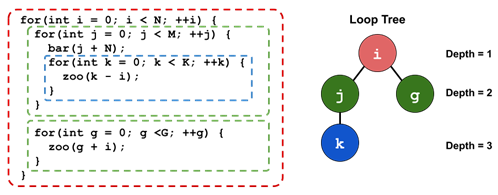
\includegraphics[width=0.8\textwidth]{content/3/chapter10/images/10.png}\\
图10.10 - 一棵循环树
\end{center}

上图中,循环\texttt{j}和\texttt{g}包围在循环\texttt{i}中,所以它们都是循环树中循环\texttt{i}的子节点。类似地,循环\texttt{k}——最内部的循环——是树中循环\texttt{j}的子节点。

循环树的根也表示函数中的顶级循环。在前面,我们学习了如何通过遍历\texttt{LoopInfo}对象来检索函数中的所有\texttt{Loop}实例——以这种方式检索的每个\texttt{Loop}实例都是顶级循环。对于给定的\texttt{Loop}实例,我们可以以类似的方式在下一层检索它的子循环。下面是一个例子:

\begin{lstlisting}[style=styleCXX]
// `LP` has the type of `Loop&`
for (Loop *SubLP : LP) {
	// `SubLP` is one of the sub-loops at the next layer
}
\end{lstlisting}

注意,前面的代码只遍历了下一层的子循环,而不是所有的后代循环。要遍历树中的所有后代循环,有两个选项:

\begin{itemize}
\item 使用\texttt{Loop::getLoopsInPreorder()}方法,可以以预先排序的方式遍历一个\texttt{Loop}实例的所有后代循环。

\item 迭代不同IR单元一节中,我们了解了什么是\texttt{GraphTraits},以及LLVM如何使用它来遍历图。LLVM也为循环树提供了一个默认的\texttt{GraphTraits}实现。因此,可以使用LLVM中现有的图迭代器遍历循环树,例如:后排序和深度优先等。下面的代码试图以深度优先的方式遍历一个以\texttt{RootL}为根的循环树:

\begin{lstlisting}[style=styleCXX]
#include "llvm/Analysis/LoopInfo.h"
#include "llvm/ADT/DepthFirstIterator.h"
…
// `RootL` has the type of `Loop*`
for (Loop *L : depth_first(RootL)) {
	// Work with `L`
}
\end{lstlisting}

在\texttt{GraphTraits}的帮助下,可以更灵活地遍历一个循环树。

\end{itemize}

除了在循环树中处理单个循环之外,LLVM还提供了一个包装器类来表示整个结构——\texttt{LoopNest}。 

\texttt{LoopNest}是由\texttt{LoopNestAnalysis}生成的分析数据。它将所有子循环封装在一个给定的\texttt{Loop}实例中,并为常用功能提供了几个“快捷”API。以下是一些重要的接口:

\begin{itemize}
\item \texttt{getOutermostLoop()}/\texttt{getInnermostLoop()}: 这些API可以哟哪里检索最外层/最内层的\texttt{Loop}实例。因为许多循环优化只适用于内部或最外层的循环,所以非常好用。

\item \texttt{areAllLoopsSimplifyForm()}/\texttt{areAllLoopsRotatedForm()}: 这些接口会表明,是否所有的循环都是某种规范形式。

\item \texttt{getPerfectLoops(…)}: 可以使用它来获得当前循环层次结构中的所有完美循环。所谓完美循环,我们指的是嵌套在一起的循环,它们之间没有“间隙”。下面是一个完美循环和非完美循环的例子:

\begin{lstlisting}[style=styleCXX]
// Perfect loops
for(int i=…) {
	for(int j=…){…}
}
// Non-perfect loops
for(int x=…) {
	foo();
	for(int y=…){…}
}
\end{lstlisting}

非完美循环的例子中,\texttt{foo}调用点是上循环和下循环之间的间隙。

许多循环优化中,完美循环是更好的选择,例如:展开完美嵌套的循环更容易——理想情况下,只需要复制最内层的循环体。

\end{itemize}

至此,我们已经了解了如何使用嵌套循环。下一节中,我们;了解学习循环优化的另一个重要主题:引导变量。

\hspace*{\fill} \\ %插入空行
\noindent
\textbf{检索引导变量的范围}

引导变量是在每次循环迭代中按特定模式前进的变量,是许多循环优化的关键。为了向量化一个循环,我们需要知道在循环中数组如何使用归纳变量——我们想要放入一个向量的数据。引导变量还可以帮助我们解决一个循环的行程计数(迭代的总次数)。在深入了解细节之前,下图展示了一些与引导变量相关的术语,以及它们在循环中的位置:

\hspace*{\fill} \\ %插入空行
\begin{center}
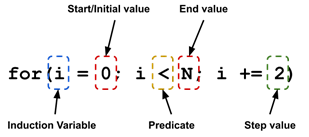
\includegraphics[width=0.6\textwidth]{content/3/chapter10/images/11.png}\\
图10.11 - 引导变量的术语
\end{center}

现在,我们来了解一些API,它们可以帮助我们检索上图中所示的组件。

首先,来讨论一下引导变量。\texttt{Loop}类已经提供了两个方便的方法来检索引导变量:\texttt{getCanoni calInductionVariable}和\texttt{getInductionVariable}。这两个方法都返回一个\texttt{PHINode}实例作为引导变量(如果有的话)。第一种方法只能在引导变量从0开始并且每次迭代只增加1的情况下使用。另一方面,第二种方法可以处理更复杂的情况,但需要一个\texttt{ScalarEvolution}实例作为参数。

\texttt{ScalarEvolution}是LLVM中一个有趣且强大的框架。简单地说,它试图跟踪值如何变化——通过算术运算——在程序路径上。将此放到循环优化的上下文中,可用于捕获循环中的递归值改变行为,这与引导变量有很强的关系。

要了解更多关于循环中引导变量的行为,可以通过\texttt{loop::getInductionDescriptor}检索\texttt{InductionDescriptor}实例。\texttt{InductionDescriptor}实例提供了一些信息,比如:初始值、步长值,以及在每次迭代时更新引导变量的指令。\texttt{Loop}类还提供了另一个类似的数据结构,用于实现引导变量的边界:\texttt{Loop::LoopBounds}类。\texttt{LoopBounds}不仅提供了引导变量的初始值和步长值,还提供了预期的结束值,以及用于检查退出条件的谓词。可以通过\texttt{Loop::getBounds}方法获取\texttt{LoopBounds}实例。

循环对程序的运行时性能至关重要。本节中,我们了解了如何在LLVM IR中表示循环,以及如何使用它们。我们还研究了它们的高级概念和各种用于检索所需循环属性的API。有了这些知识,我们就离创建更有效、更积极的循环优化和从目标应用程序获得更高的性能更近了一步。













